%!TeX root =  ../../thesis.tex

\section{Arduino}
Pro účely vytvoření testeru na kabely byl vybrán mikrokontrolér od značky Arduino model \ardMeg. Tento model disponuje velkým počtem pinům, jak digitálních tak analogových, které budou potřeba vzhledem k potřebám testeru. Já použiji pouze ty digitální pro připojení konektorů pro testování kabelů, klávesnice a bzučáku. Mikrokontrolér Arduino se dá programovat pomocí mnoha jazyků, zejména pak C/C++.

\begin{figure}[H]
	\centering
	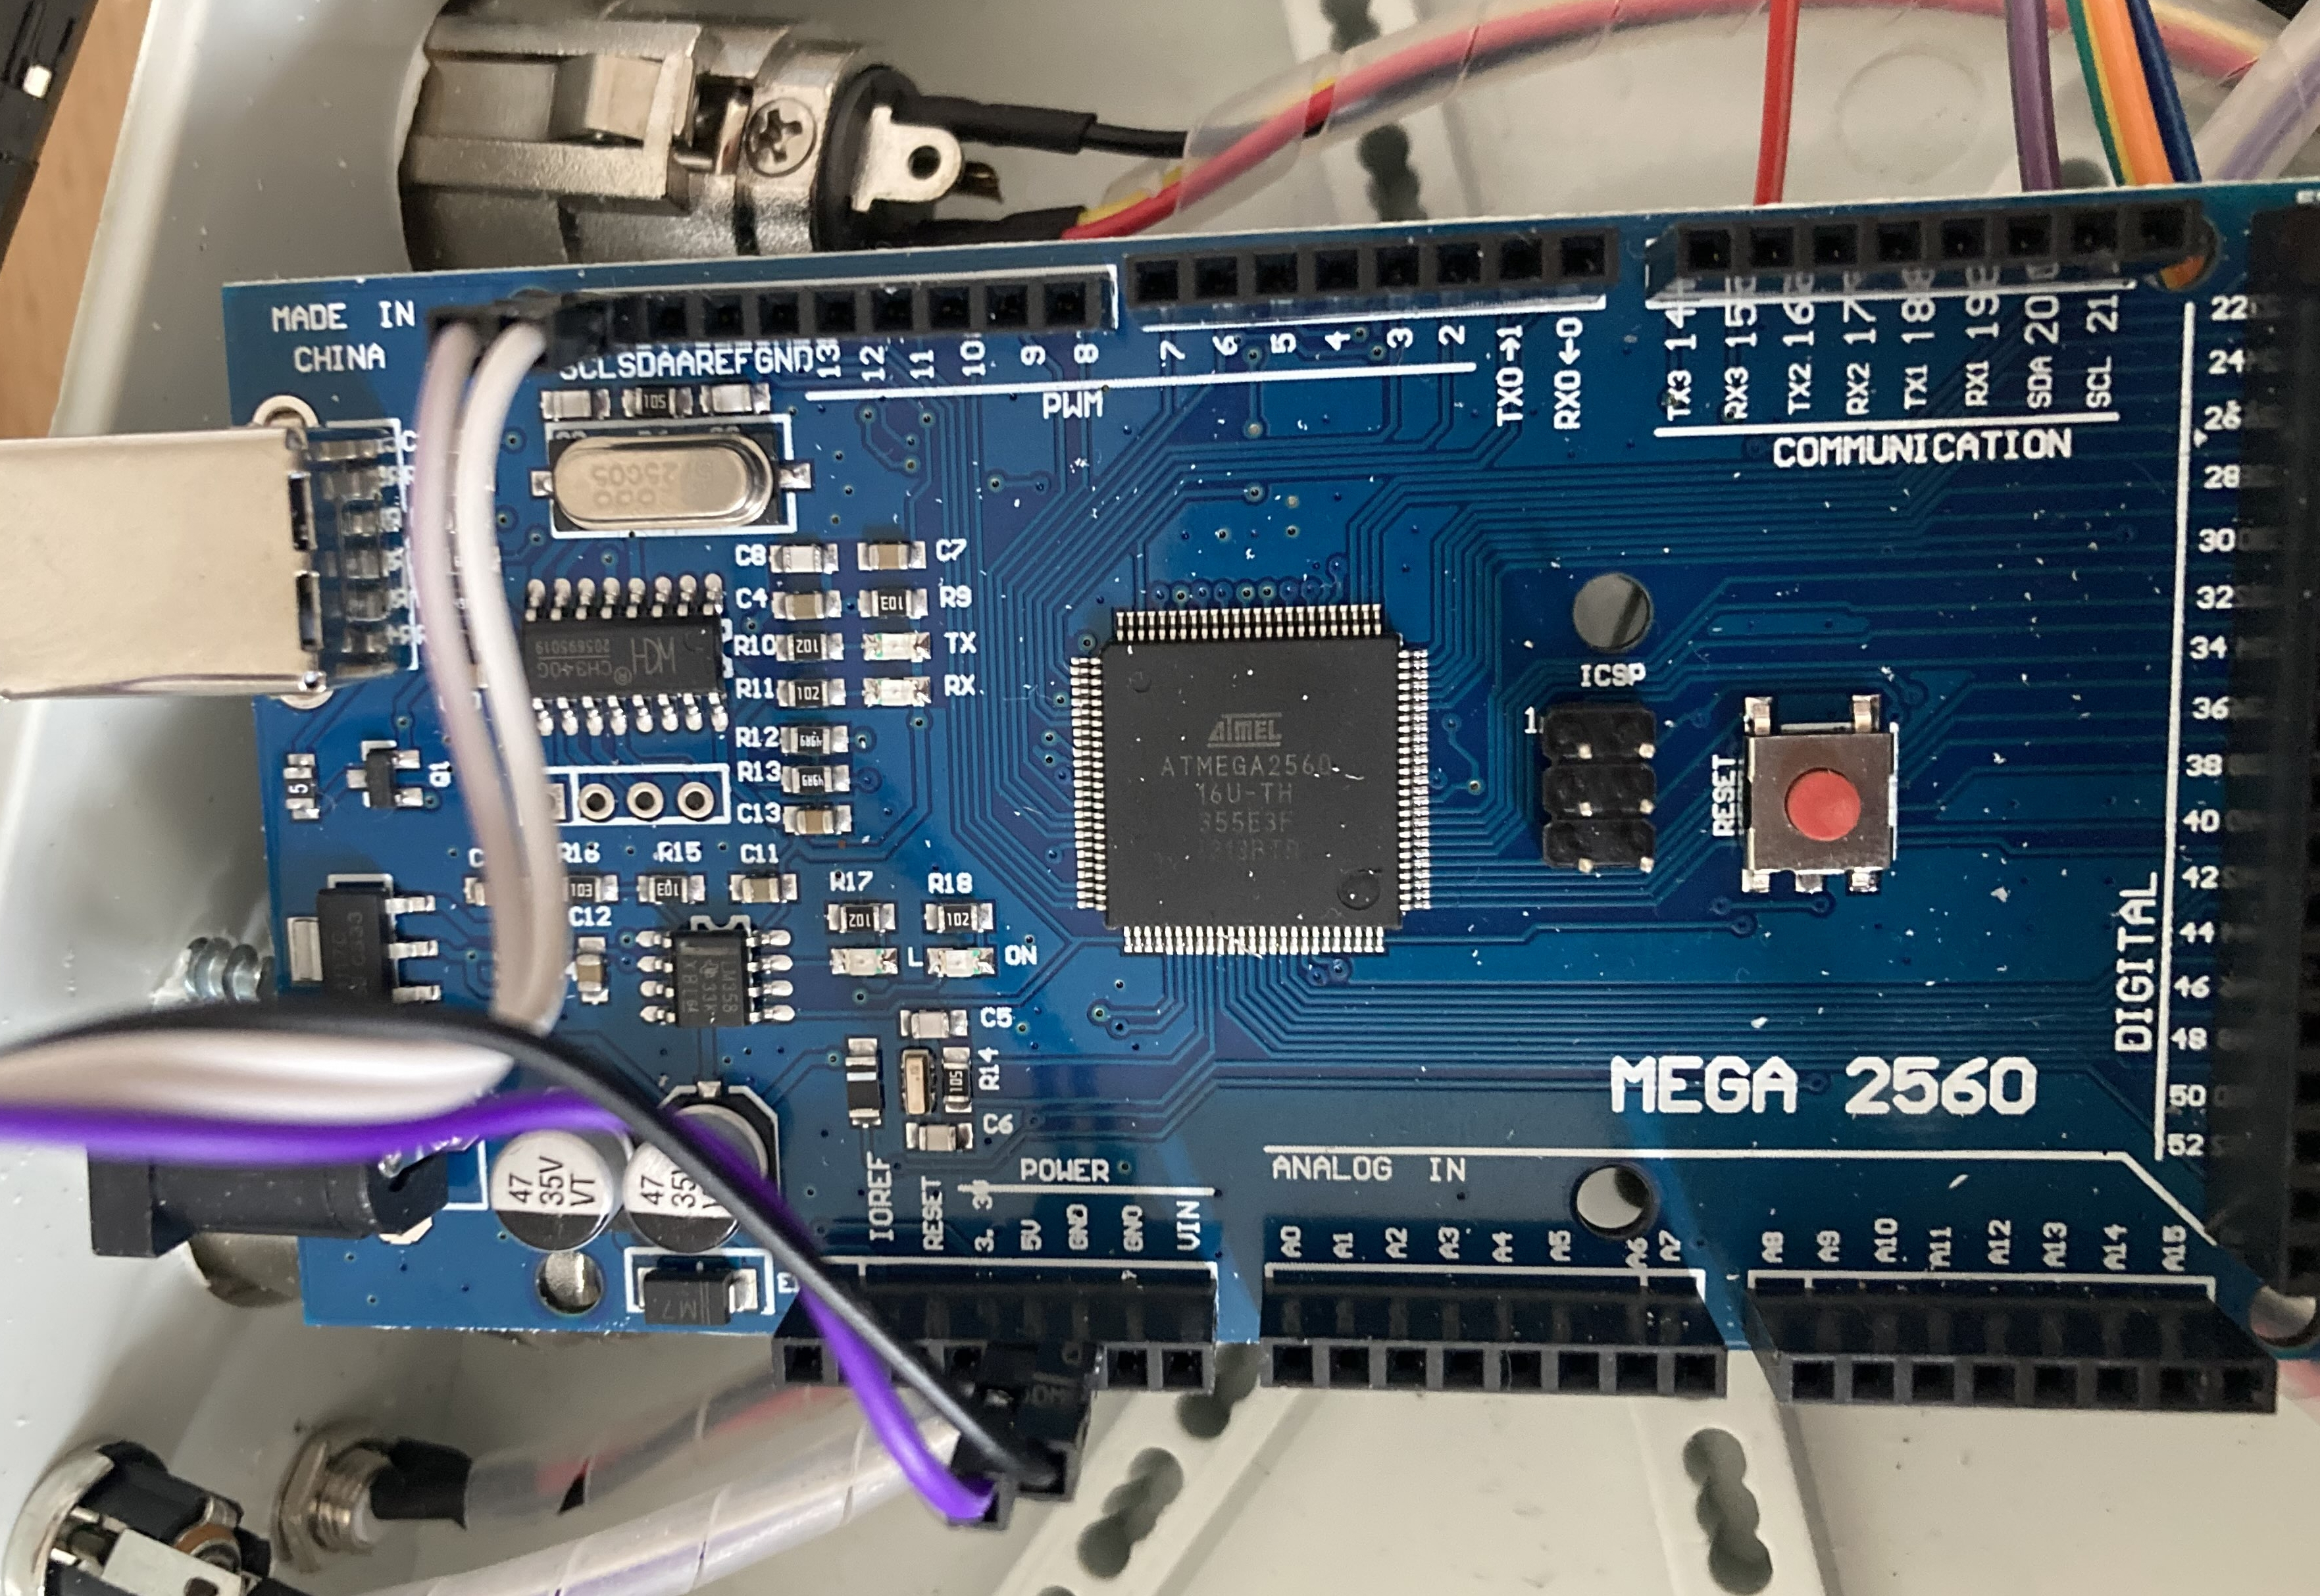
\includegraphics[width=0.9\textwidth]{pictures/megaBoard.jpg}
    	\caption{\ardMeg}
   	\label{fig:arduinoMega}
\end{figure}

Na obrázku \ref{fig:arduinoMega} je deska, která je klon Arduina, ale je plně kompatibilní s Arduino softwarem i hardwarem, jelikož je Arduino open source, tak jsou tyto klony běžné a jsou i o dost levnější. Každopádně tato deka je shodná s \ardMeg.